% !TEX spellcheck = en_US

% !TEX root = elastophi-report.tex

\section*{Introduction}

This document aims at presenting the work achieved for project Elasto$\Phi$ during the CEMRACS summer school  
that took place at the Centre International de Rencontres Math\'ematiques (CIRM) at Luminy from July 24th to 
August 25th, 2016. This project originated from mathematical challenges encountered by IFP Energies Nouvelles (IFPEN)
for the numerical solution of an elastostatic problem in an infinite homogeneous background medium containing crack 
networks with highly complex geometrical structure, see Figure~\ref{fig:structureExamples}. 

\begin{figure}[hb]
\centering
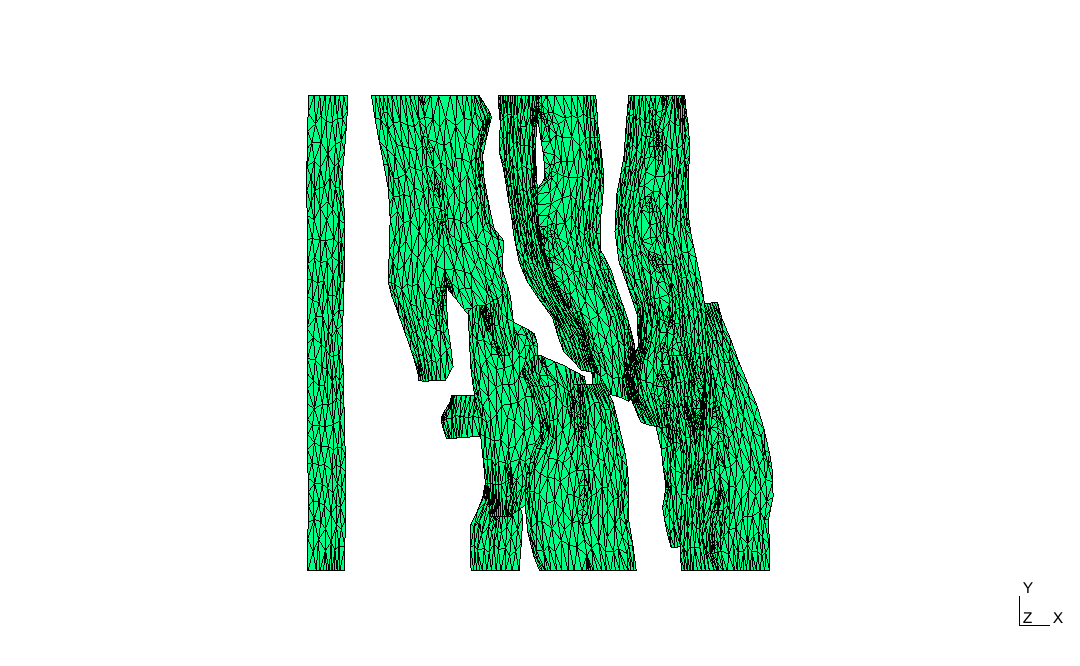
\includegraphics[width=0.4\textwidth]{../images/visu_maillage5364FracsTriangles.png} \qquad 
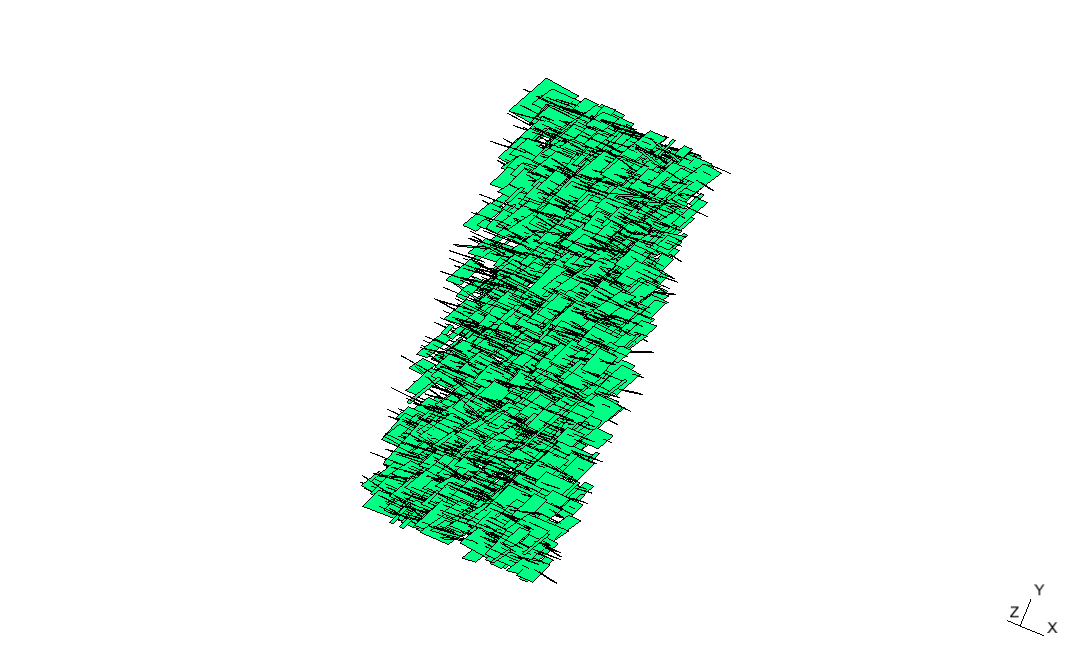
\includegraphics[width=0.3\textwidth]{../images/visu_maillage1994Fracs.png}
\caption{Examples of crack networks.}
\label{fig:structureExamples}
\end{figure}

\bigskip
This problem was reformulated as boundary integral equation posed at the surface of cracks, and 
discretized by means of Galerkin procedure based on piecewise constant functions, which is commonly known as 
Boundary Element Method (BEM). The fully non-local structure of boundary integral operators leads to  
densely populated matrices. As a consequence, if the matrix of the problem is of size $N$, 
then any matrix-vector product (which is the most elementary building block of any iterative linear solver)
requires at least $\mathcal{O}(N^{2})$ operations.

\bigskip
As in most industrial applications, for the problems considered by IFPEN this situation is not acceptable. 
Indeed, computational complexity of $N^{2}$ makes it impossible to perform a matrix-vector product for $N$ larger than
say $10^{6}$: this would be too costly in terms of time and memory storage. At the same time, the  applications 
considered by IFPEN typically require $N$ to be of this order.

\bigskip
To deal with this difficulty, IFPEN developed a heuristic method consisting in forcing coefficients of the 
BEM matrix to zero whenever this coefficient corresponds to the interaction between sufficiently distant points 
of the crack network. With this procedure, the matrix of the problem is approximated by a sparsified matrix that 
allows matrix-vector products with $\mathcal{O}(N)$ complexity. But this strategy also induces substantial consistency 
error: measured in Frobenius norm, the perturbation on the matrix is typically between $16$\% and $40$\% large.

\bigskip
On the other hand, current literature on boundary integral equation nowadays offers a panel of refined complexity reduction 
techniques: fast multipole methods, hierarchical matrix strategies, and the like. These techniques, that have been developed 
during the last two decades, have been introduced to accelerate computations in a wide variety of problems ranging from molecular 
dynamics \cite{?}, to astrophysics \cite{?}. Acceleration of boundary integral equations on smooth surfaces has also been 
historically a key challenge for stimulating the development of such methods \cite{?}.

\bigskip
The main goal of the CEMRACS project Elasto$\Phi$ was to test the performance of one of these reduction techniques on the 
crack network problem of IFPEN. Although the above mentioned complexity reduction techniques are particularly well suited  
for boundary integral equations, the problem under consideration from IFPEN was not just a straightforward application of 
the state of the art, because it involves a strongly irregular geometry. Besides development issues, this was the main 
challenging  aspect of the project.

\bigskip
The Elasto$\Phi$ project mainly consisted in developing a numerical mockup code in C++ and testing it on the matrices sent 
by IFPEN. We implemented one particular complexity reduction technique: Hierarchical Matrix \cite{?} format combined with the Adaptative Cross 
Approximation (ACA) compression method \cite{?}. For the sake of brevity, we shall refer to this approach as HM-ACA. We could not test several 
complexity reduction techniques, this would have required more time (CEMRACS is only 5 weeks long\dots). Among all complexity reduction techniques 
already available (multipoles, panel clustering, etc\dots), we chose HM-ACA because this was the only approach that treats generation 
of the matrix of the problem in a black-box manner. All other methods are far more intrusive, and most of the time their development 
is also more time consuming. On the other hand, due to confidentiality restrictions, we did not have access to the source code of IFPEN, and 
in particular could not actually get the routine generating the coefficients of the matrix. These constraints led us to choose HM-ACA.

\bigskip
There already exist freely accessible libraries written in C or C++ that implement HM-ACA, see e.g.~HLib (\url{http://hlib.org/}), H2Lib 
(\url{http://www.h2lib.org/}) or Ahmed (\url{https://github.com/xantares/ahmed}),  but they are poorly documented. Besides IFPEN required 
that the code numerical mockup developed during the project can be reused by IFPEN after the CEMRACS summer school, 
and the license of all existing libraries was incompatible with this condition. For these reasons, we decided to redevelop simply  
a "homemade" implementation of HM-ACA. The code that we developed was put under Lesser Gnu Public License (LGPL) and 
put on a Github repository freely accessible at
\begin{center}
\url{https://github.com/xclaeys/ElastoPhi}
\end{center}

\medskip
The outline of this report is as follows. We will first describe the Adaptative Cross Approximation method, and show its efficiency 
for the compression of dense matrices admitting fast decreasing singular values (such matrices shall be referred to in the sequel as admissible). 
Unfortunately the matrices generated by boundary element  methods (and in particular the matrices considered by IFPEN) do not have 
fast decreasing eigenvalues. We shall then comment on this point, describing the problem and the boundary integral equation 
considered by IFPEN. Since the ACA compression method is not directly applicable, we are led to decompose the matrix in sub-blocks, 
each of which is either small or admissible. To be efficient, such a decomposition has to follow certain rules, and in particular 
admit a hierarchical structure. Such a technique, that we shall then describe, is referred to as a "hierarchical matrix format". 
Then we shall give a detailed overview of the code developed during the project, and conclude the report by a series of test 
cases where we report the performances of our code.


\section{Low rank approximations}
\label{sec:LowRankApprox}

In this section we are interested in fully populated matrices $\mA\in \C^{n\times n}$, $\mA = (\mA_{j,k})_{j,k=1\dots n}$ with, a priori, 
none of its entries vanishing, its size $n$ being potentially large. With no particular assumption on this matrix, the cost of a 
matrix-vector product is $\mathcal{O}(n^{2})$. 

\bigskip
This cost is substantially reduced if we assume that $\mA$ is of low rank though. We say that a matrix has the low rank property, 
with rank $k\leq n$, if there exist vectors $\bfu_{j},\bfv_{j}\in \C^{n}, j=1\dots k$, such that 
$$
\mA = \sum_{j=1}^{k}\bfu_{j}\cdot\bfv_{j}^{T}\quad \textrm{with}\quad k\leq n/2.
$$ 
Indeed if this representation holds, then a matrix-vector product requires $2 k n$ flops, which is smaller than $n^{2}$ provided 
that the condition on $k$ given above is satisfied. Matrices $\mA$ encountered in applications rarely have the low rank property. 
A simple primary observation is that general matrices $\mA$ can be written as a sum of rank one matrices through its singular value
decomposition
\begin{equation}\label{SVD}
\mA = \sum_{j=1}^{n}\sigma_{j}\,\bfu_{j}\cdot\bfv_{j}^{T}\quad \textrm{where}\;\; \mathfrak{S}(\mA^{*}\mA) = \{\sigma_{j}^{2}\}_{j=1\dots n},
\end{equation}
where $(\bfu_{j})_{j=1}^{n}, (\bfv_{j})_{j=1}^{n}$ are orthonormal basis of $\C^{n}$ and $\sigma_{1}\geq \sigma_{2}\geq \dots \geq \sigma_{n}$. 
A closer inspection of this formula leads to the conclusion, provided that the sequence $(\sigma_{j})$  decreases fast, that 
truncating the singular value decomposition (\ref{SVD}) yields a good approximation of the matrix $\mA$. This is the essence of 
the next result.

\begin{proposition}\quad\\
Let $\mA\in \C^{n\times n}$ admit the singular value decomposition (\ref{SVD}), and denote $\mA_{k}$ the 
matrix obtained by truncating this decomposition at rank $k$ namely $\mA_{k}:=\sum_{j=1}^{k}\sigma_{j}\,\bfu_{j}
\cdot\bfv_{j}^{T}$. Then we have the error estimates
$$
\Vert \mA - \mA_{k}\Vert_{2}^{2} = \sigma_{k+1}^{2}
\quad\textrm{and}\quad 
\Vert \mA - \mA_{k}\Vert_{\mrm{F}}^{2} = \sum_{j=k+1}^{n}\sigma_{j}^{2}
$$
where $\Vert \;\Vert_{2}$ refers to the matrix norm induced by the vector norm $\vert \bfu\vert_{2} = (\sum_{j=1}^{n}\vert u_{j}\vert^{2})$ 
for $\bfu = (u_{j})_{j=1}^{n}\in \C$ and $\Vert \;\Vert_{\mrm{F}}$ refers to the Fr\"obenius norm.
\end{proposition}

Truncating the SVD is thus an efficient way to approximate a matrix, and thus to reduce the cost of the 
matrix-vector product, provided that  the singular values decrease fast. Assume that singular values decrease 
exponentially, say $\sigma_{k}\leq q^{k}$ for a fixed $q\in (0,1)$. Then for a relative error expressed in Fr\"obenius norm of order $\varepsilon>0$,  
it suffices to take $k \simeq \log_q \varepsilon$. 

\bigskip
Unfortunately, computing the singular value decomposition  of a matrix is expensive: it costs $\mathcal{O}(n^{3})$ flops. To circumvent this issue, starting from 
an arbitrary matrix $\mA$ whose singular values are assumed to decrease exponentially, the Adaptative 
Cross Approximation algorithm provides a collection of vectors $\bfu_{j},\bfv_{j}\in \C^{n}, j=1\dots n$ such that 
the matrices $\widetilde{\mA}_{k} = \sum_{j=1}^{k}\bfu_{j}\cdot\bfv_{j}^{T}$ satisfy 
$$
\Vert \mA - \widetilde{\mA}_{k}\Vert_{\mrm{F}}\leq C \Vert \mA - \mA_{k}\Vert_{\mrm{F}}
$$
for some constant $C>0$ independent of $k$. Moreover, which is probably the most interesting feature of this method, 
the cost of computing $\widetilde{\mA}_{k}$ is $\mathcal{O}(kn)$. This cost is thus quasi-linear provided that the singular 
values  decrease exponentially. The detailed analysis of the ACA algorithm is out of the scope of this report. We only 
give the algorithm itself.

\begin{algorithm}\label{AlgoACA}
  \caption{Partially Pivoted ACA}
  Initialize $j_{*}$\\
  $r=0$\\
  \textbf{while}(stopping criterion not satisfied)\{\\\quad\\
  \indent\hspace{0.5cm} \parbox{\linewidth}{
    $\bfw = \mA(j_{*},:)^{T} - \sum_{\ell=1}^{r}\bfu_{\ell}(j_{*})\,\bfv_{\ell}$\\
    $k_{*} = \mathop{\mrm{argmax}}_{k = 1\dots n}\vert \bfw(k)\vert$\\
    $w_{*} = \bfw(k_{*})$\\\quad\\
    \textbf{if}($w_{*}\neq 0$)\{\\\quad\\
    \indent\hspace{0.5cm} \parbox{\linewidth}{
      $\bfv_{r+1} = \bfw$\\
      $\bfw = \mA(:,k_{*})-\sum_{\ell = 1}^{r}\bfv_{\ell}(k_{*})\,\bfu_{\ell} $\\
      $\bfu_{r+1} = w_{*}^{-1}\bfw$\\      
      $j_{*} = \mathop{\mrm{argmax}}_{j = 1\dots n} \vert \bfw(j)\vert$\\
      $r=r+1$
    }
    \quad\\
    \}\\\quad\\
    \textbf{else}\{terminate algorithm\}
    }\\
  \}
\end{algorithm}

\bigskip
In our pseudo-code notation, for any vector $\bfw\in \C^{n}$, the number $\bfw(j)$  refers to the $j$th entry of $\bfw$. 
Likewise for $\mA\in \C^{n\times n}$, the number $\mA(:,k)$ refers to the $k$th column, and $\mA(j,:)$ refers to the $j$th
row.

\bigskip
At the beginning of Algorithm \ref{AlgoACA}, there is an initialization step for the choice of the index of the first $j_{*}$. 
For this initialization, one could take $j_{*} = 1$. Other choices may speed up the convergence of the algorithm. Such heuristics 
are problem dependent. Algorithm \ref{AlgoACA} also involves a stopping criterion based on an error estimator. During the Elasto$\Phi$ 
project, we took the stopping criterion given in \cite{...Rjasanow-Steinbach}
$$
\begin{array}{l}
\textbf{Stopping criterion:}\\ 
\vert \bfu_{r}\vert_{2}\vert \bfv_{r}\vert_{2}\leq  \varepsilon\Vert \sum_{\ell = 1}^{r}\bfu_{\ell}\cdot\bfv_{\ell}^{T}\Vert_{\mrm{F}}\\[10pt]
\textrm{where}\quad \Vert \sum_{\ell = 1}^{r}\bfu_{\ell}\cdot\bfv_{\ell}^{T}\Vert_{\mrm{F}}^{2} = \sum_{j=1}^{r}\sum_{k=1}^{r}
(\overline{\bfu}_{j}^{T}\bfu_{k})(\overline{\bfv}_{j}^{T}\bfv_{k}).
\end{array}
$$
\textcolor{red}{
In this stopping criterion, the value $\varepsilon>0$ is a fitting parameter whose choice depends on the degree of consistency 
that one wishes. Due to the requirements of IFPEN in terms of consistency, we typically chose values 
$\varepsilon = 1e-1$ or $1e-2$.
}


\section{The matrix under consideration}\label{sec:GalerkinMatrix}

We now shall give some more details about the matrices under consideration during the Elasto$\Phi$ project. 
As previously mentioned, these matrices stemmed from a Galerkin discretization of a boundary integral 
equation. Assume that $\Gamma$ is a surface embedded in $\R^{3}$ that is the union of a collection 
$\mathcal{T} = \{\tau_{j}\}_{j=1}^{N}$ of flat triangles and quadrangles
$$
\Gamma = \mathop{\bigcup}_{j=1}^{N}\tau_{j}\;,\quad\quad \tau_{j} = \textrm{triangle or quadrangle}.
$$
The elements $\tau_{j}$ might intersect each other, which makes $\Gamma$ a potentially very rough surface.
Let us briefly describe the bilinear form associated with the variational formulation under consideration for 
the Galerkin discretization. We need to introduce the Green kernel of the problem, that is given by the explicit formula 
$$
\mathscr{G}(\bx) = \frac{1}{8\pi E}\frac{1+\rho}{1-\rho}\biggl( \frac{3-4\rho}{\vert \bx\vert}\mrm{Id}  +\frac{\bx\cdot\bx^{T}}{\vert \bx\vert^{3}}\biggr).
$$
It is fundamental to observe, and to keep in mind, that this function is singular at $\bx = 0$. In this expression, $\rho$ 
refers to the Poisson ratio, and $E$ is the elasticity module. Next, for each element $\tau$, let  $\bn_{\tau}$ refer to a vector field 
normal to $\tau$, and for any vector field $\bu\colon\Gamma\to \R^{3}$, define the trace operator
$$
\begin{array}{l}
\dsp{ \mathscr{R}_{\tau}(\bu) = \lambda\bn_{\tau}\div(\bu)+2\mu\,(\bn_{\tau}\cdot\nabla)\bu + \mu\bn_{\tau}\times\curl(\bu), }\\[10pt]
\dsp{ \textrm{with}\quad \lambda := \frac{E\rho}{(1+\mu)(1-2\rho)},\quad \mu := \frac{E}{2(1+\rho)}}.
\end{array}
$$
The variational formulation associated with the problem under consideration typically consists in finding $\bu\in \mH^{1/2}_{00}(\Gamma)^{3}$ 
such that $a(\bu,\bv) = f(\bv)$ for all $\bv\in \mH^{1/2}_{00}(\Gamma)^{3}$, where $\mH^{1/2}_{00}(\Gamma):=\Pi_{\tau\in\mathcal{T}}\mH^{1/2}_{00}(\tau)^{3}$
and the bilinear form is given by
\begin{equation}\label{VariationnalFormulation}
\begin{array}{l}
\dsp{ a(\bu,\bv) = \sum_{\tau\in\mathcal{T}}\sum_{\tau'}\int_{\tau\times\tau'}\mathscr{R}_{\tau}^{\by}(\mathscr{R}_{\tau'}^{\bx}\mathscr{G}(\bx-\by)) \bu(\bx)\bv(\by) d\sigma(\bx) d\sigma(\by).  }
\end{array}
\end{equation}
In this formula the operator $\mathscr{R}_{\tau}^{\bx}$ is the operator $\mathscr{R}_{\tau}$ applied with respect the $\bx$ variable. The operator $\mathscr{R}_{\tau'}^{\by}$ 
is defined accordingly. Formula  (\ref{VariationnalFormulation}) is rather abstract. Another, more explicit expression of this operator can be obtained, 
see e.g.~\cite{??}, but this is pointless for the present report. The only important thing here is that the integral kernel coming into play in this integral 
operator is singular at $\bx = \by$ (which is possible only if $\tau\cap \tau'\neq \emptyset$), and it is regular otherwise. In particular, if $\tau$ and $\tau'$
are distant from each other, then the operator associated with $a(\;,\;)$ is regularizing, and it will induce matrices with exponentially decreasing singular values.
Now let us describe how the bilinear form (\ref{VariationnalFormulation}) is discretized. Each space $\mH^{1/2}_{00}(\tau)^{3}$ is approximated with a three dimensional 
space 
$$
\mH_{h}(\tau)\simeq \mH^{1/2}_{00}(\tau)^{3}\quad \mrm{dim}(\mH_{h}(\tau)) = 3\quad \textrm{for each}\;\;\tau\in \mathcal{T}.
$$ 
Next the global variational space is obtained by a simple cartesian product $\mH_{h}(\Gamma) = \Pi_{\tau\in \mathcal{T}}\mH_{h}(\tau)$.
Finally the discrete variational formulation writes: find $\bu_{h}\in \mH_{h}(\Gamma)$ such that 
\begin{equation}\label{discreteVF}
a(\bu_{h},\bv_{h}) = f(\bv_{h})\quad \bv_{h}\in \mH_{h}(\Gamma).
\end{equation}
Following the classical Galerkin discretization procedure, a matrix is derived from (\ref{discreteVF}) simply by specifying a basis for 
$\mH_{h}(\Gamma)$. In the present case, such a basis is specified as follows. Denote $\bpsi_{3j-2}(\bx), \bpsi_{3j-1}(\bx),\bpsi_{3j}(\bx)$ 
three vector fields  generating $\mH_{h}(\tau_{j})$ (recall that $\mrm{dim}(\mH_{h}(\tau_{j}) )= 3$ by hypothesis). Then we have 
$$
\mH_{h}(\Gamma) = \mathop{\mrm{span}}_{j=1\dots 3N}\{\bpsi_{j}\}.
$$
Of course, here, each $\bpsi_{3j-q}$ with $q=0,1,2$ is regarded as a function defined on $\Gamma$ that is supported 
only on $\tau_{j}$. Then the matrices that we had to deal with during Project Elatso$\Phi$ are defined as 
$\mA = (\mA_{j,k})_{j,k=1\dots 3N}$ where 
\begin{equation}\label{GalerkinMatrix}
\mA_{j,k}:=a(\bpsi_{j},\bpsi_{k}),\quad j,k = 1\dots 3N.
\end{equation}


\section{Partition of the matrix in admissible blocks}

In the sequel, for any subsets $t,s\subset \llbr1,3N\rrbr$, let $\mA_{t,s}$ refer to the sub-block extracted from $\mA$ 
by restricting indices to the set $t\times s$. We define $\mA_{b}$ similarly for any $b\subset \llbr 1,3N\rrbr\times \llbr 1,3N\rrbr$.

\bigskip
Two important conclusions should be drawn from the discussion of the previous paragraph. The first 
conclusion is that, due to the singularity of the integral kernel, the singular values of the matrix given 
by (\ref{GalerkinMatrix}) do \textit{not} decrease exponentially i.e.~this matrix is not admissible. 
As a consequence, the ACA compression strategy of Section \ref{sec:LowRankApprox} is not directly applicable 
to this matrix. 

\bigskip
However sub-blocks of the matrix $\mA$ given by (\ref{GalerkinMatrix}) may be admissible (i.e.~have exponentially 
decreasing singular values). To build an approximation of $\mA$ allowing a substantial reduction of the cost of 
matrix-vector products, it would be sufficient to find a sparse matrix $\mA_{\mrm{sp}}\in \C^{3N\times 3N}$ such that 
$$
\mA = \mA_{\mrm{sp}} + \sum_{t\times s\in \mathscr{B}} \mA_{b}
$$
where $\mathscr{B}$ is a partition of $\llbr 1,3N\rrbr\times \llbr 1,3N\rrbr$ \textcolor{red}{into $\mathcal{O}(N\log N)$}, and each 
$\mA_{b}$ is admissible. Indeed with such a decomposition, one may consider $\mA' = \mA_{\mrm{sp}} + \sum_{t\times s\in \mathscr{B}} \mA_{b}'$
as a good approximation for $\mA$, where each $\mA_{b}'$ is obtained from $\mA_{b}$ after application of the ACA compression 
procedure described in Section \ref{sec:LowRankApprox}. In this manner, keeping $\mathcal{O}(1)$ terms (i.e.~a few terms) from each 
ACA compression procedure the cost of a matrix-vector product is now $\mathcal{O}(N\log N)$.


\bigskip
The second conclusion that can be drawn from the discussion of Section \ref{sec:GalerkinMatrix} is that the Galerkin discretization establishes 
a correspondence between the numbering of unknowns on the one end, and some spatial distribution of degrees of freedom. This gives insight 
on how to find admissible (and thus compressible) sub-blocks inside the matrix $\mA$, as follows.

For a ball $\mB_{s}\subset \R^{3}$, define $s = \{j \in\llbr 1,3N\rrbr\;\vert \;\mrm{supp}(\bpsi_{j})\subset \mB_{s}\}$. 
For another ball $\mB_{t}\subset \R^{3}$, define $t\subset \llbr1,3N\rrbr$ accordingly.  
The more $\mB_{s}$ and $\mB_{t}$ are far from each other, the faster the singular values of $\mA_{t,s}$ will decrease. 

The distance between $\mB_{t}$ and $\mB_{s}$ that may considered as sufficient depends on the radius of these balls. 
Such a criterion shall be referred later on as \textit{admissibility criterion}. Current literature provides various 
admissibility criterion. It should be considered as problem dependent. For the project Elasto$\Phi$, we considered the 
following admissibility criterion (see \cite{...Rjasanow - Steinbach})
\begin{equation}\label{AdmissibilityCondition}
\mrm{min}\big( \mrm{diam}(\mB_{t}),\mrm{diam}(\mB_{s})\big)< \eta\;\mrm{dist}(\mrm{B}_{t},\mrm{B}_{s}),
\end{equation}
where $\eta>0$ is a fitting parameter. For the present problem, the typical values of $\eta$ that we considered  
range from $\eta = 0.1$ to $\eta = 10$.






